%%%%%%%%%%%%%%%%%%%%%%%%%%%%%%%%%%%%%%%%%%%%%%%%%%%%%%%%%%%%%%%%%%%%%%%%%%%%%%%%
\subsection{Συμπεράσματα κεφαλαίου}
\label{subsection:02_02_05:01}

Σε αυτό το κεφάλαιο μάς απασχόλησε η ελάττωση του σφάλματος εκτίμησης στάσης
με αιτία τα ευρήματά μας στο προηγούμενο κεφάλαιο
(ενότητα \ref{subsection:02_01_05:02}). Με δεδομένο τη χρήση του φίλτρου
σωματιδίων για το έργο της παρακολούθησης της στάσης ενός ρομπότ, αναλύσαμε τη
διαθέσιμη βιβλιογραφία γύρω από την ελάττωση του σφάλματος εκτίμησης του, και
προτείναμε δύο επιπρόσθετους τρόπους με τους οποίους είναι δυνατή η επίτευξη
του στόχου. Πιο συγκεκριμένα:

\begin{itemize}
  \item Επικεντρωθήκαμε στο μοντέλο παρατηρήσεων του φίλτρου, και, σκεπτόμενοι
        αναλυτικά, θέσαμε την υπόθεση ότι η επιλογή υποσυνόλων από υποθέσεις
        στάσης του, των οποίων οι αναμενόμενες μετρήσεις από αυτές συμβαδίζουν
        περισσότερο με τις εισερχόμενες στο φίλτρο μετρήσεις του αισθητήρα
        αποστάσεων σε σχέση με άλλες υποθέσεις---η επιλογή αυτών των υποθέσεων
        στάσης ως η εκτίμηση του φίλτρου οφείλει να παράγει χαμηλότερα σφάλματα
        στάσης (ενότητα \ref{subsection:02_02_03:01}). Τα ευρήματά μας
        επιβεβαιώνουν την υπόθεση, αλλά έως ένα κατώφλι πληθικότητας αυτών των
        υποσυνόλων: στο όριο, η μοναδική υπόθεση στάσης που εμφανίζει τη
        μεγαλύτερη πιθανότητα παρατήρησης των μετρήσεων από αυτήν εμφανίζει
        μεγαλύτερα σφάλματα στάσης από ότι η συλλογική εκτίμηση του φίλτρου.
        Βάσει αυτού του ευρήματος συμπεράναμε ότι το φίλτρο σωματιδίων δεν
        αποτελεί άθροισμα υποθέσεων, αλλά μία κατακερματισμένη μορφή εκτίμησης.
  \item Ερευνήσαμε και ζητήσαμε να ελέγξουμε την ευστάθεια της υπόθεσης ότι
        το αποτέλεσμα της εφαρμογής του μετασχηματισμού της ευθυγράμμισης
        μετρήσεων δισδιάστατου αισθητήρα lidar με σαρώσεις χάρτη από την
        παραγώμενη εκτίμηση του φίλτρου στην ίδια την εκτίμηση του εμφανίζει
        χαμηλότερα σφάλματα εκτίμησης στάσης σε σχέση με την αρχική εκτίμηση
        (ενότητα \ref{subsection:02_02_03:02}). Με βάση τη διαμόρφωση της
        πειραματικής διαδικασίας, τα ευρήματα αποδεικνύουν ότι η εφαρμογή της
        διαδικασίας ευθυγράμμισης έχει σημαντικά οφέλη στην ελάττωση του
        σφάλματος εκτίμησης.
  \item Παρακινούμενοι από ελλείψεις και μεινοκτήματα μεθόδων της τρέχουσας
        βιβλιογραφίας προτείναμε έναν τρόπο ανάδρασης του αποτελέσματος της
        ευθυγράμμισης μετρήσεων με σαρώσεις χάρτη στον πληθυσμό του φίλτρου
        σωματιδίων (ενότητα \ref{subsection:02_02_03:03}): δεδομένων ότι το
        αποτέλεσμα της ευθυγράμμισης (α) είναι πιο ακριβές από την εκτίμηση του
        φίλτρου και (β) είναι άγνωστο στο ίδιο το φίλτρο, σχεδιάσαμε έναν
        μηχανισμό ανάδρασης που (i) προκαλεί πιο γρήγορη σύγκλιση και
        χαμηλότερα σφάλματα εκτίμησης σε σχέση με έναν μηχανισμό ανάδρασης της
        βιβλιογραφίας, (ii) προκαλεί την αποφυγή απόκλισης του φίλτρου σε σχέση
        με έναν δεύτερο μηχανισμό ανάδρασης της βιβλιογραφίας, και (iii)
        εμφανίζει χαμηλότερα σφάλματα στάσης σε σχέση με το φίλτρο σε κατάσταση
        ανοιχτού βρόχου.
\end{itemize}

Στο σχήμα \ref{fig:02_02_05:01} απεικονίζονται συνοπτικά οι συμβολές του
παρόντος κεφαλαίου στη μεθοδολογία ελάττωσης του σφάλματος εκτίμησης φίλτρου
σωματιδίων με χρήση αισθητήρων απόστασης τύπου 2D lidar.

\begin{figure}
  \hspace{-1.5cm}
  % GNUPLOT: LaTeX picture with Postscript
\begingroup
  \makeatletter
  \providecommand\color[2][]{%
    \GenericError{(gnuplot) \space\space\space\@spaces}{%
      Package color not loaded in conjunction with
      terminal option `colourtext'%
    }{See the gnuplot documentation for explanation.%
    }{Either use 'blacktext' in gnuplot or load the package
      color.sty in LaTeX.}%
    \renewcommand\color[2][]{}%
  }%
  \providecommand\includegraphics[2][]{%
    \GenericError{(gnuplot) \space\space\space\@spaces}{%
      Package graphicx or graphics not loaded%
    }{See the gnuplot documentation for explanation.%
    }{The gnuplot epslatex terminal needs graphicx.sty or graphics.sty.}%
    \renewcommand\includegraphics[2][]{}%
  }%
  \providecommand\rotatebox[2]{#2}%
  \@ifundefined{ifGPcolor}{%
    \newif\ifGPcolor
    \GPcolorfalse
  }{}%
  \@ifundefined{ifGPblacktext}{%
    \newif\ifGPblacktext
    \GPblacktexttrue
  }{}%
  % define a \g@addto@macro without @ in the name:
  \let\gplgaddtomacro\g@addto@macro
  % define empty templates for all commands taking text:
  \gdef\gplfronttext{}%
  \makeatother
  \ifGPblacktext
    % no textcolor at all
    \def\colorrgb#1{}%
    \def\colorgray#1{}%
  \else
    % gray or color?
    \ifGPcolor
      \def\colorrgb#1{\color[rgb]{#1}}%
      \def\colorgray#1{\color[gray]{#1}}%
      \expandafter\def\csname LTw\endcsname{\color{white}}%
      \expandafter\def\csname LTb\endcsname{\color{black}}%
      \expandafter\def\csname LTa\endcsname{\color{black}}%
      \expandafter\def\csname LT0\endcsname{\color[rgb]{1,0,0}}%
      \expandafter\def\csname LT1\endcsname{\color[rgb]{0,1,0}}%
      \expandafter\def\csname LT2\endcsname{\color[rgb]{0,0,1}}%
      \expandafter\def\csname LT3\endcsname{\color[rgb]{1,0,1}}%
      \expandafter\def\csname LT4\endcsname{\color[rgb]{0,1,1}}%
      \expandafter\def\csname LT5\endcsname{\color[rgb]{1,1,0}}%
      \expandafter\def\csname LT6\endcsname{\color[rgb]{0,0,0}}%
      \expandafter\def\csname LT7\endcsname{\color[rgb]{1,0.3,0}}%
      \expandafter\def\csname LT8\endcsname{\color[rgb]{0.5,0.5,0.5}}%
    \else
      % gray
      \def\colorrgb#1{\color{black}}%
      \def\colorgray#1{\color[gray]{#1}}%
      \expandafter\def\csname LTw\endcsname{\color{white}}%
      \expandafter\def\csname LTb\endcsname{\color{black}}%
      \expandafter\def\csname LTa\endcsname{\color{black}}%
      \expandafter\def\csname LT0\endcsname{\color{black}}%
      \expandafter\def\csname LT1\endcsname{\color{black}}%
      \expandafter\def\csname LT2\endcsname{\color{black}}%
      \expandafter\def\csname LT3\endcsname{\color{black}}%
      \expandafter\def\csname LT4\endcsname{\color{black}}%
      \expandafter\def\csname LT5\endcsname{\color{black}}%
      \expandafter\def\csname LT6\endcsname{\color{black}}%
      \expandafter\def\csname LT7\endcsname{\color{black}}%
      \expandafter\def\csname LT8\endcsname{\color{black}}%
    \fi
  \fi
  \setlength{\unitlength}{0.0500bp}%
  \begin{picture}(10000.00,4000.00)%
    \gplgaddtomacro\gplfronttext{%
      \colorrgb{0.00,0.00,0.00}%
      \put(1168,440){\makebox(0,0)[r]{\strut{}$0.005$}}%
      \colorrgb{0.00,0.00,0.00}%
      \put(1168,1526){\makebox(0,0)[r]{\strut{}$0.010$}}%
      \colorrgb{0.00,0.00,0.00}%
      \put(1168,2613){\makebox(0,0)[r]{\strut{}$0.015$}}%
      \colorrgb{0.00,0.00,0.00}%
      \put(1300,220){\makebox(0,0){\strut{}$200$}}%
      \colorrgb{0.00,0.00,0.00}%
      \put(2091,220){\makebox(0,0){\strut{}$600$}}%
      \colorrgb{0.00,0.00,0.00}%
      \put(2882,220){\makebox(0,0){\strut{}$1000$}}%
      \colorrgb{0.00,0.00,0.00}%
      \put(5000,4600){\makebox(0,0){\strut{}Μέσο σφάλμα εκτίμησης σε $N = 100$ διαδρομές ανά εκτιμώμενη στάση}}%
      \colorrgb{0.00,0.00,0.00}%
      \put(5100,-510){\makebox(0,0){\strut{}Αριθμός εκτιμήσεων στάσης στο χρόνο}}%
      \definecolor{gr}{RGB}{161,214,107}
      \definecolor{pi}{RGB}{232,163,201}
      \definecolor{k}{RGB}{0,0,0}
      \definecolor{sm}{RGB}{227,74,51}
      \put(2110,4229){\makebox(0,0){\strut{}{\color{k}{\rule[0.6mm]{0.5cm}{0.5mm}}} MCL}}
      \put(2200,4000){\makebox(0,0){\strut{}{\color{gr}{\rule[0.6mm]{0.5cm}{0.5mm}}} $\%$MCL}}
      \put(1900,4000){\makebox(0,0){\strut{}{\color{pi}{\rule[0.6mm]{0.25cm}{0.5mm}}}}}

      \put(4700,4229){\makebox(0,0){\strut{}{\color{k}{\rule[0.6mm]{0.5cm}{0.5mm}}} MCL}}
      \put(5100,4000){\makebox(0,0){\strut{}{\color{sm}{\rule[0.6mm]{0.5cm}{0.5mm}}} MCL $\circ$ smsm}}

      \put(7460,4229){\makebox(0,0){\strut{}{\color{k}{\hdashrule[0.6mm]{0.60cm}{0.5mm}{0.5mm}}} MCL}}
      \put(8100,4000){\makebox(0,0){\strut{}{\color{k}{\rule[0.6mm]{0.5cm}{0.5mm}}} MCL $\circ$ smsm $\circ$ $\circlearrowleft$}}

      \put(2210,-100){\makebox(0,0){\strut{} CORRIDOR}}
      \put(5000,-100){\makebox(0,0){\strut{} WAREHOUSE}}
      \put(7990,-100){\makebox(0,0){\strut{} WAREHOUSE}}
    }%
    \gplgaddtomacro\gplfronttext{%
    }%
    \gplgaddtomacro\gplfronttext{%
      \colorrgb{0.00,0.00,0.00}%
      \put(4053,440){\makebox(0,0)[r]{\strut{}$0$}}%
      \colorrgb{0.00,0.00,0.00}%
      \put(4053,1092){\makebox(0,0)[r]{\strut{}$0.02$}}%
      \colorrgb{0.00,0.00,0.00}%
      \put(4053,1744){\makebox(0,0)[r]{\strut{}$0.04$}}%
      \colorrgb{0.00,0.00,0.00}%
      \put(4053,2395){\makebox(0,0)[r]{\strut{}$0.06$}}%
      \colorrgb{0.00,0.00,0.00}%
      \put(4053,3047){\makebox(0,0)[r]{\strut{}$0.08$}}%
      \colorrgb{0.00,0.00,0.00}%
      \put(4053,3699){\makebox(0,0)[r]{\strut{}$0.10$}}%
      \colorrgb{0.00,0.00,0.00}%
      \put(4185,220){\makebox(0,0){\strut{}$0$}}%
      \colorrgb{0.00,0.00,0.00}%
      \put(4734,220){\makebox(0,0){\strut{}$100$}}%
      \colorrgb{0.00,0.00,0.00}%
      \put(5284,220){\makebox(0,0){\strut{}$200$}}%
      \colorrgb{0.00,0.00,0.00}%
      \put(5833,220){\makebox(0,0){\strut{}$300$}}%
    }%
    \gplgaddtomacro\gplfronttext{%
      \colorrgb{0.00,0.00,0.00}%
      \put(6939,440){\makebox(0,0)[r]{\strut{}$0$}}%
      \colorrgb{0.00,0.00,0.00}%
      \put(6939,1092){\makebox(0,0)[r]{\strut{}$0.02$}}%
      \colorrgb{0.00,0.00,0.00}%
      \put(6939,1744){\makebox(0,0)[r]{\strut{}$0.04$}}%
      \colorrgb{0.00,0.00,0.00}%
      \put(6939,2395){\makebox(0,0)[r]{\strut{}$0.06$}}%
      \colorrgb{0.00,0.00,0.00}%
      \put(6939,3047){\makebox(0,0)[r]{\strut{}$0.08$}}%
      \colorrgb{0.00,0.00,0.00}%
      \put(6939,3699){\makebox(0,0)[r]{\strut{}$0.10$}}%
      \colorrgb{0.00,0.00,0.00}%
      \put(7071,220){\makebox(0,0){\strut{}$0$}}%
      \colorrgb{0.00,0.00,0.00}%
      \put(7620,220){\makebox(0,0){\strut{}$100$}}%
      \colorrgb{0.00,0.00,0.00}%
      \put(8170,220){\makebox(0,0){\strut{}$200$}}%
      \colorrgb{0.00,0.00,0.00}%
      \put(8719,220){\makebox(0,0){\strut{}$300$}}%
    }%
    \put(0,0){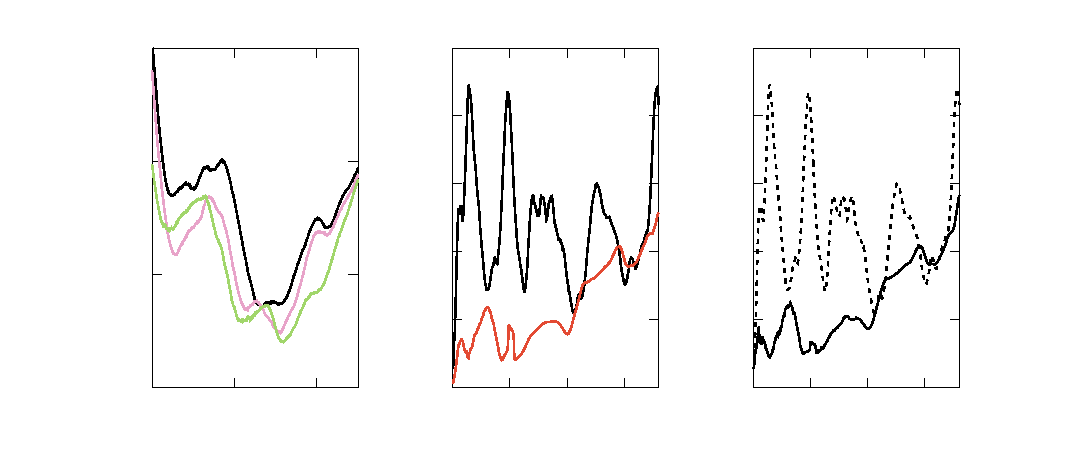
\includegraphics{./figures/parts/02/chapters/02/sections/05/h_123}}%
    \gplfronttext
  \end{picture}%
\endgroup

  \vspace{1cm}
  \caption{\small Η συμβολή των μεθόδων που παρουσιάστηκαν στο παρόν κεφάλαιο
           ως προς το μέσο σφάλμα εκτίμησης ανά στάση στα διενεργηθέντα
           πειράματα. Αριστερά: με μαύρο χρώμα το αποτέλεσμα του MCL και με άλλα
           χρώματα το αποτέλεσμα της επιλογής υποσυνόλων σωματιδίων στο
           περιβάλλον CORRIDOR. Μέση: με μαύρο χρώμα το αποτέλεσμα του MCL και
           με κόκκινο το αποτέλεσμα της ευθυγράμμισης μετρήσεων δισδιάστατου
           αισθητήρα lidar με σαρώσεις χάρτη (smsm). Δεξιά: με διακεκομμένη
           γραμμή το αποτέλεσμα του MCL και με συνεχή το αποτέλεσμα του ολικού
           συστήματος (σχήμα \ref{fig:overall_system}) μετά την ανατροφοδότηση
           του αποτελέσματος της ευθυγράμμισης μετρήσεων με σαρώσεις χάρτη
           στον πληθυσμό του φίλτρου μέσω της προτεινόμενης μεθόδου
           ανατροφοδότησης}
  \label{fig:02_02_05:01}
\end{figure}


%%%%%%%%%%%%%%%%%%%%%%%%%%%%%%%%%%%%%%%%%%%%%%%%%%%%%%%%%%%%%%%%%%%%%%%%%%%%%%%%
\subsection{Αιτίες περαιτέρω έρευνας}
\label{subsection:02_02_05:02}

Η κυριότερη αιτία και το πιο γόνιμο έδαφος για περαιτέρω έρευνα αφορά στη
μέθοδο ευθυγράμμισης δισδιάστατων μετρήσεων αισθητήρα lidar με σαρώσεις χάρτη.
Κατά τη διάρκεια διεξαγωγής της υλοποίησης του σύνθετου συστήματος περάσαμε από
το στάδιο ενσωμάτωσης μίας εκ των υλοποιήσεών της, ήτοι του PLICP, και, προτού
την ενσωματώσουμε οριστικά στο σύνθετο σύστημα, την υποβάλαμε σε μία σειρά από
δοκιμές ώστε να επαληθεύσουμε τη ορθότητά των αποτελεσμάτων που εμφανίζονται
στη βιβλιογραφία και αφορούν σε αυτήν, αλλά στα συμφραζόμενα της έρευνας μας.
Κατά τη διάρκεια αυτών των δοκιμών καταλήξαμε σε μία σειρά από πορίσματα που
στηρίζουν το συμπέρασμα της πρώτης πρότασής μας, τα οποία παρουσιάζουμε
παρακάτω.

Ένα κύριο πρόβλημα---αν όχι το κυριότερο---στο οποίο πρέπει να δοθεί προσοχή
όσο αφορά στους αλγορίθμους ευθυγράμμισης σαρώσεων είναι η πρακτική της εύρεσης
αντιστοιχίσεων ανάμεσα στις ακτίνες των εισόδων τους. Αυτό αφορά σε όλες τις
προσεγγίσεις ευθυγραμμίσεων σαρώσεων με σαρώσεις (πραγματικών μετρήσεων με
πραγματικές μετρήσεις ή με εικονικές μετρήσεις από χάρτη), και όχι μόνο στη
μέθοδο ICP και την πληθώρα των παραλλαγών της. Το πρόβλημα εδώ είναι ότι,
δεδομένου του θορύβου του αισθητήρα μέτρησης και των αποκλίσεων μεταξύ του
χάρτη και περιβάλλοντος που αναπαριστά, η δημιουργία αντιστοιχίσεων μπορεί να
οδηγήσει σε ανακριβή αποτελέσματα ή συνολικά σε αποκλίνοντα αποτελέσματα. Στην
πράξη, όσον αφορά στις μεθόδους που λειτουργούν απευθείας στο χώρο των
μετρήσεων, η αντιστοίχιση πραγματοποιείται μέσω διαδικασιών που εξαρτώνται από
την ικανοποίηση παραδοχών-υποθέσεων, και από την ακριβή ρύθμιση εξωτερικά
παρεχόμενων παραμέτρων. Αυτές οι παράμετροι περιλαμβάνουν, για παράδειγμα, την
εκτίμηση της τυπικής απόκλισης του κανονικά κατανεμημένου θορύβου μηδενικής
μέσης τιμής που επιδρά στις μετρήσεις ενός αισθητήρα αποστάσεων---όταν οι
μετρήσεις του αισθητήρα μπορεί στην πραγματικότητα να είναι μεροληπτικές
(biased), ή να μην ικανοποιούν την παραδοχή της κανονικής κατανομής του θορύβου
τους \cite{Cooper2018a}---, ή την εκτίμηση του ποσοστού των ακτίνων που δεν
αντιστοιχούν σε άλλες μεταξύ των εισόδων τους (κάτι που είναι εκ των προτέρων
θεμελιωδώς άγνωστο και αδύνατο να εκτιμηθεί).

Αυτό μας οδηγεί σε ένα άλλο κρίσιμο σημείο: το ζήτημα της παραμετροποίησης. Η
επίδοση της πλειονότητας των μεθόδων ευθυγράμμισης σάρωσης στηρίζεται στον
ακριβή καθορισμό της τιμής των παραμέτρων που διέπουν τις εσωτερικές τους
διαδικασίες. Γενικά, θεωρείται ορθά ότι οι εν λόγω παράμετροι πρέπει να
καθορίζονται για ένα συγκεκριμένο περιβάλλον και για συγκεκριμένο επίπεδο
θορύβου, αλλά στην πραγματικότητα, ελλείψει αυτόματης ρύθμισης των παραμέτρων,
διαφορετικές παραμετροποιήσεις μπορεί να οδηγήσουν σε ασταθή ή μη διαισθητικά
αποτελέσματα---και το αποτέλεσμα αυτό μπορεί να εμφανιστεί ακόμη και για την
ίδια στάση στο ίδιο περιβάλλον. Θα αποσαφηνίσουμε αυτές τις ιδιότητες με ένα
απλό αλλά χαρακτηριστικό παράδειγμα.

\begin{figure}\centering
  % GNUPLOT: LaTeX picture with Postscript
\begingroup
  \makeatletter
  \providecommand\color[2][]{%
    \GenericError{(gnuplot) \space\space\space\@spaces}{%
      Package color not loaded in conjunction with
      terminal option `colourtext'%
    }{See the gnuplot documentation for explanation.%
    }{Either use 'blacktext' in gnuplot or load the package
      color.sty in LaTeX.}%
    \renewcommand\color[2][]{}%
  }%
  \providecommand\includegraphics[2][]{%
    \GenericError{(gnuplot) \space\space\space\@spaces}{%
      Package graphicx or graphics not loaded%
    }{See the gnuplot documentation for explanation.%
    }{The gnuplot epslatex terminal needs graphicx.sty or graphics.sty.}%
    \renewcommand\includegraphics[2][]{}%
  }%
  \providecommand\rotatebox[2]{#2}%
  \@ifundefined{ifGPcolor}{%
    \newif\ifGPcolor
    \GPcolorfalse
  }{}%
  \@ifundefined{ifGPblacktext}{%
    \newif\ifGPblacktext
    \GPblacktexttrue
  }{}%
  % define a \g@addto@macro without @ in the name:
  \let\gplgaddtomacro\g@addto@macro
  % define empty templates for all commands taking text:
  \gdef\gplfronttext{}%
  \gdef\gplfronttext{}%
  \makeatother
  \ifGPblacktext
    % no textcolor at all
    \def\colorrgb#1{}%
    \def\colorgray#1{}%
  \else
    % gray or color?
    \ifGPcolor
      \def\colorrgb#1{\color[rgb]{#1}}%
      \def\colorgray#1{\color[gray]{#1}}%
      \expandafter\def\csname LTw\endcsname{\color{white}}%
      \expandafter\def\csname LTb\endcsname{\color{black}}%
      \expandafter\def\csname LTa\endcsname{\color{black}}%
      \expandafter\def\csname LT0\endcsname{\color[rgb]{1,0,0}}%
      \expandafter\def\csname LT1\endcsname{\color[rgb]{0,1,0}}%
      \expandafter\def\csname LT2\endcsname{\color[rgb]{0,0,1}}%
      \expandafter\def\csname LT3\endcsname{\color[rgb]{1,0,1}}%
      \expandafter\def\csname LT4\endcsname{\color[rgb]{0,1,1}}%
      \expandafter\def\csname LT5\endcsname{\color[rgb]{1,1,0}}%
      \expandafter\def\csname LT6\endcsname{\color[rgb]{0,0,0}}%
      \expandafter\def\csname LT7\endcsname{\color[rgb]{1,0.3,0}}%
      \expandafter\def\csname LT8\endcsname{\color[rgb]{0.5,0.5,0.5}}%
    \else
      % gray
      \def\colorrgb#1{\color{black}}%
      \def\colorgray#1{\color[gray]{#1}}%
      \expandafter\def\csname LTw\endcsname{\color{white}}%
      \expandafter\def\csname LTb\endcsname{\color{black}}%
      \expandafter\def\csname LTa\endcsname{\color{black}}%
      \expandafter\def\csname LT0\endcsname{\color{black}}%
      \expandafter\def\csname LT1\endcsname{\color{black}}%
      \expandafter\def\csname LT2\endcsname{\color{black}}%
      \expandafter\def\csname LT3\endcsname{\color{black}}%
      \expandafter\def\csname LT4\endcsname{\color{black}}%
      \expandafter\def\csname LT5\endcsname{\color{black}}%
      \expandafter\def\csname LT6\endcsname{\color{black}}%
      \expandafter\def\csname LT7\endcsname{\color{black}}%
      \expandafter\def\csname LT8\endcsname{\color{black}}%
    \fi
  \fi
  \setlength{\unitlength}{0.0500bp}%
  \begin{picture}(4000.00,4000.00)%
    \gplgaddtomacro\gplfronttext{%
      \colorrgb{0.00,0.00,0.00}%
      \put(388,877){\makebox(0,0)[r]{\strut{}$4$}}%
      \colorrgb{0.00,0.00,0.00}%
      \put(388,1354){\makebox(0,0)[r]{\strut{}$6$}}%
      \colorrgb{0.00,0.00,0.00}%
      \put(388,1831){\makebox(0,0)[r]{\strut{}$8$}}%
      \colorrgb{0.00,0.00,0.00}%
      \put(388,2307){\makebox(0,0)[r]{\strut{}$10$}}%
      \colorrgb{0.00,0.00,0.00}%
      \put(388,2784){\makebox(0,0)[r]{\strut{}$12$}}%
      \colorrgb{0.00,0.00,0.00}%
      \put(388,3261){\makebox(0,0)[r]{\strut{}$14$}}%
      \colorrgb{0.00,0.00,0.00}%
      \put(520,419){\makebox(0,0){\strut{}$2$}}%
      \colorrgb{0.00,0.00,0.00}%
      \put(997,419){\makebox(0,0){\strut{}$4$}}%
      \colorrgb{0.00,0.00,0.00}%
      \put(1474,419){\makebox(0,0){\strut{}$6$}}%
      \colorrgb{0.00,0.00,0.00}%
      \put(1950,419){\makebox(0,0){\strut{}$8$}}%
      \colorrgb{0.00,0.00,0.00}%
      \put(2427,419){\makebox(0,0){\strut{}$10$}}%
      \colorrgb{0.00,0.00,0.00}%
      \put(2904,419){\makebox(0,0){\strut{}$12$}}%
      \colorrgb{0.00,0.00,0.00}%
      \put(3381,419){\makebox(0,0){\strut{}$14$}}%
      \colorrgb{0.00,0.00,0.00}%
      \put(-118,2069){\rotatebox{90}{\makebox(0,0){\strut{}$y$ [m]}}}%
      \colorrgb{0.00,0.00,0.00}%
      \put(2069,89){\makebox(0,0){\strut{}$x$ [m]}}%
      \put(2800,2700){\makebox(0,0){\strut{}$\bm{x}_a$}}%
      \put(1090,2200){\makebox(0,0){\strut{}$\bm{x}_b$}}%
      \put(1690,2500){\makebox(0,0){\strut{}$\bm{x}_c$}}%
    }%
    \gplgaddtomacro\gplfronttext{%
    }%
    \put(0,0){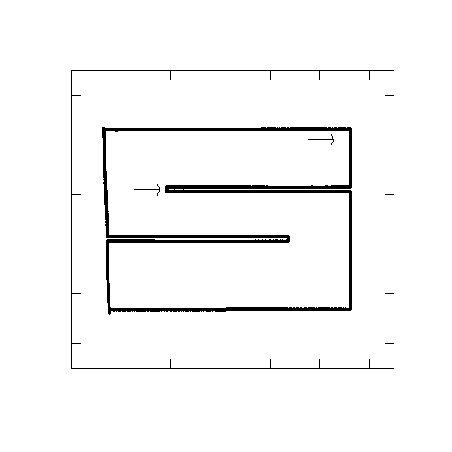
\includegraphics{./figures/parts/02/chapters/02/sections/05/corridor_motivation}}%
    \gplfronttext
  \end{picture}%
\endgroup

  \caption{\small Ο χάρτης του περιβάλλοντος CORRIDOR, $\bm{M}_C$, και δύο
           στάσεις μέσα σε αυτόν, $\bm{x}_a(11.56, 12.2, 0.0)$, και
           $\bm{x}_b(4.56, 10.2, 0.0)$}
  \label{fig:02_02_05:corridor_motivation}
\end{figure}

Στο σχήμα \ref{fig:02_02_05:corridor_motivation} παρουσιάζεται ο χάρτης του μη
σύνθετου περιβάλλοντος CORRIDOR, $\bm{M}_C$, στο οποίο πραγματοποιήσαμε έναν
αριθμό πειραμάτων ευθυγράμμισης μετρήσεων lidar με σαρώσεις χάρτη, με τη χρήση
ενός πανοραμικού αισθητήρα δισδιάστατων μετρήσεων και τον αλγόριθμο
ευθυγράμμισης PLICP. Η πειραματική διαδικασία είναι η εξής: μέσα στον ελεύθερο
χώρο του χάρτη διασπείρεται ένας αριθμός από υποθέσεις στάσεων, ενώ η
πραγματική στάση του αισθητήρα τίθεται ως $\bm{x}_a$ ή $\bm{x}_b$. Στη συνέχεια
πραγματοποιούνται τόσες ευθυγραμμίσεις μετρήσεων με σαρώσεις χάρτη όσες αυτές
οι υποθέσεις, ανάμεσα στη μέτρηση του πραγματικού αισθητήρα, που λαμβάνεται από
την πραγματική του στάση, και εικονικές σαρώσεις που λαμβάνονται από τις
στάσεις των υποθέσεων. Ως τελική εκτίμηση λαμβάνεται η διορθωμένη στάση της
υπόθεσης για την οποία το σφάλμα ευθυγράμμισης (εξ. \ref{eq:sm_def}) καταγράφει
τη μικρότερη τιμή ανάμεσα σε όλες τις διορθώσεις των στάσεων-υποθέσεων. Ένα
αρχικό σύνολο παραμέτρων αποτελεί τη βάση από την οποία τροποποιούνται $8$
βασικές παράμετροι για μία φορά και στη συνέχεια τίθενται στην προεπιλεγμένη
τιμή τους. Προκειμένου να ερευνηθεί η συμπεριφορά του PLICP εκτελέσαμε την
παραπάνω πειραματική διαδικασία για τις στάσεις $\bm{x}_a$ και $\bm{x}_b$, και
δύο διαφορετικά επίπεδα θορύβου, με σταθερό αριθμό σταθερών στάσεων-υποθέσεων,
για $10$ φορές, διενεργώντας έτσι $N = 2 \times 2 \times 14 \times 10 = 560$
πειράματα. Η τοποθέτηση των στάσεων διατηρήθηκε σταθερή ώστε να είναι δυνατή η
εκτέλεση άμεσων συγκρίσεων ανάμεσα σε όλες τις διαμορφώσεις. Ο πίνακας
\ref{tbl:csm_diff_params} απεικονίζει τις παραμέτρους υπό τροποποίηση και το
συνολικό σφάλμα στάσης για κάθε λύση.  Λεπτοµέρειες σχετικά µε τη σηµασία και
τη χρήση κάθε παραμέτρου βρίσκονται στα \cite{csm_manual1} και
\cite{csm_manual2}.


\begin{table*}\centering
\begin{tabular}{lccrrrrr}

  & & & \multicolumn{5}{c}{Σφάλμα στάσης} \\
                                      &                 &                 & \multicolumn{2}{c}{$\|\bm{e}(\bm{x}_a,\hat{\bm{x}}_a^\ast)\|_2$} &          & \multicolumn{2}{c}{$\|\bm{e}(\bm{x}_b,\hat{\bm{x}}_b^\ast)\|_2$} \\ \toprule
  Θόρυβος μέτρησης $\mathcal{N}(0,\sigma)$, $\sigma$: & &                 & $0.0$             & $0.01$        &  & $0.0$            & $0.01$     \\
  Αρχικό σύνολο παραμέτρων            &                 &                 & $0.0065$        & $0.0056$        &  & $0.0368$         & $0.0377$   \\
  Τροποποιημένη παράμετρος            & Τιμή            & Αρχική          &                 &                 &  &                  &            \\ \midrule
  \texttt{use\_corr\_tricks}          & \texttt{true}   & \texttt{false}  & $0.0065$        & $0.0064$        &  & $0.0368$         & $0.0377$   \\
  \texttt{restart}                    & \texttt{true}   & \texttt{false}  & $0.0065$        & $0.0074$        &  & $0.0368$         & $0.0377$   \\
  \texttt{clustering\_threshold}      & $1.025$         & $0.025$         & $0.0065$        & $0.0060$        &  & $0.0368$         & $0.0381$   \\
  \texttt{do\_alpha\_test}            & \texttt{false}  & \texttt{true}   & $0.0065$        & $0.0069$        &  & $0.0368$         & $0.0384$   \\
  \texttt{orientation\_neighbourhood} & $2$             & $20$            & $0.0065$        & $0.0066$        &  & $0.0368$         & $0.0372$   \\
                                      & $200$           &                 & $15.425$        & $15.425$        &  & $9.9153$         & $9.9153$   \\
  \texttt{outliers\_maxPerc}          & $0.9$           & $1.0$           & $0.0043$        & $0.0060$        &  & $0.0357$         & $0.0358$   \\
                                      & $0.8$           &                 & $0.0044$        & $0.0051$        &  & $0.0359$         & $0.0384$   \\
                                      & $0.7$           &                 & $4.7091$        & $0.0047$        &  & $10.298$         & $0.0377$   \\
  \texttt{outliers\_adaptive\_order}  & $0.9$           & $1.0$           & $0.0044$        & $0.0047$        &  & $0.0355$         & $0.0363$   \\
                                      & $0.8$           &                 & $0.0043$        & $0.0057$        &  & $0.0366$         & $0.0368$   \\
                                      & $0.7$           &                 & $0.0042$        & $0.0040$        &  & $2.9225$         & $4.4985$   \\
  \texttt{outliers\_remove\_doubles}  & \texttt{true}   & \texttt{false}  & $0.0062$        & $0.0064$        &  & $0.0362$         & $0.0367$   \\ \bottomrule
\end{tabular}
  \caption{\small Το σφάλμα στάσης $\|\bm{e}(\bm{x},\hat{\bm{x}}^\ast)\|_2$ της
           διορθωμένης υπόθεσης $\hat{\bm{x}}^\ast$ η οποία εμφανίζει το
           χαμηλότερο σφάλμα ευθυγράμμισης που βρέθηκε από τον PLICP στο
           περιβάλλον CORRIDOR (εικ.  \ref{fig:02_02_05:corridor_motivation})
           σε $N$ πειράματα, για ένα προεπιλεγμένο σύνολο παραμέτρων και για
           διαφορετικές τιμές βασικών παραμέτρων, και δύο επίπεδα θορύβου του
           αισθητήρα, ο οποίος υποτίθεται ότι είναι κανονικά κατανεμημένος με
           τυπική απόκλιση $\sigma$ [m]. Η μονάδα του μέτρησης του σφάλματος
           στάσης είναι $(\text{m}^2+\text{rad}^2)^{1/2}$}
\label{tbl:csm_diff_params}
\end{table*}


Θα ξεκινήσουμε την ανάλυση της άστατης συμπεριφοράς του PLICP εστιάζοντας στα
αποτελέσματα που αφορούν στην ευθυγράμμιση ελλείψει μετρητικού θορύβου. Για τις
δύο συγκεκριμένες στάσεις, του συγκεκριμένου περιβάλλοντος, η τροποποίηση των
παραμέτρων που σχετίζονται με τη χρήση ενισχυμένων μεθόδων εύρεσης
αντιστοιχίσεων (\texttt{use\_corr\_tricks}), την επανεκκίνηση όταν μια λύση
υπερβαίνει ένα κατώφλι (\texttt{restart}), την ομαδοποίηση σημείων
(\texttt{clustering\_threshold}), τη δοκιμή μιας λύσης λαμβάνοντας υπόψη τον
προσανατολισμό του κάθετου στην επιφάνεια των σαρώσεων διανύσματος
(\texttt{do\_alpha\_test}), και τον αριθμό των γειτονικών ακτίνων που
χρησιμοποιούνται για την εκτίμηση του προσανατολισμού
(\texttt{orientation\_neighbourhood})---η τροποποίηση αυτών των παραμέτρων
έχει μηδενική επίδραση στη λύση του αλγορίθμου, για κάθε στάση του
αισθητήρα. Εάν εξετάσουμε το σφάλμα στάσης σε σχέση με αυτές τις παραμέτρους
όταν υπάρχει θόρυβος τότε παρατηρούμε ότι η τροποποίηση μιας παραμέτρου μπορεί
να έχει θετικό αντίκτυπο στη λύση για μια στάση, αλλά αρνητικό για άλλη
(π.χ. \texttt{use\_corr\_tricks}, \texttt{clustering\_threshold}). Επιπλέον, η
τροποποίηση παραμέτρων που αφορούν σε λειτουργικότητες των οποίων ο σκοπός
είναι η βελτίωση της επίδοσης της μεθόδου δεν οδηγεί πάντα στο επιθυμητό
αποτέλεσμα (π.χ. \texttt{use\_corr\_tricks}, \texttt{restart}). Η τροποποίηση
άλλων παραμέτρων προς τη θετική κατεύθυνση (δηλαδή τροποποίηση που έχει ως
σκοπό τη μείωση του σφάλματος ευθυγράμμισης, π.χ.
\texttt{outliers\_remove\_doubles}) παράγει συνεπή αποτελέσματα για όλα τα
επίπεδα θορύβου των μετρήσεων του αισθητήρα για μια στάση ($\bm{x}_b$), ασυνεπή
για άλλα ($\bm{x}_a$), ή συνολικά καταστροφικά λανθασμένα αποτελέσματα
(\texttt{orientation\_neighbourhood} $=200$).

Η υψηλότερη ευαισθησία των λύσεων του PLICP, ωστόσο, παρουσιάζεται όσον αφορά
παραμέτρους που σχετίζονται με το φιλτράρισμα των μη έγκυρων αντιστοιχίσεων, οι
οποίες συμβολίζονται με το πρόθεμα \texttt{outliers\_}. Η τιμή
$1.0-$\texttt{outliers\_maxPerc} καθορίζει το ποσοστό των αντιστοιχίσεων με το
μεγαλύτερο σφάλμα που πρέπει να απορρίφθούν, ενώ η τιμή
\texttt{outliers\_adaptive\_order} καθορίζει το κατώτερο ποσοστό των
αντιστοιχίσεων (ανάλογα με το σφάλμα τους) για το οποίο εκτελείται
προσαρμοστικός (adaptive) αλγόριθμος για την απόρριψη τους. Όσον αφορά στην
πρώτη παράμετρο, αυτό που παρατηρούμε και για τις δύο πραγματικές στάσεις του
αισθητήρα είναι ότι η απόρριψη του κορυφαίου $30\%$ των πιο λανθασμένων
αντιστοιχίσεων οδηγεί σε καταστροφική αποτυχία ελλείψει θορύβου, αλλά ακριβή
συμπεριφορά στην αντίθετη περίπτωση. Όσον αφορά σε άλλες τιμές, δεν
παρατηρείται συνεπής συμπεριφορά, αν και όλες οδηγούν σε σωστή σύγκλιση. Όσον
αφορά στη δεύτερη παράμετρο, η ασυνέπεια μεταξύ των αποτελεσμάτων προκύπτει στο
επίπεδο διαφορετικών στάσεων---η ρύθμιση αυτής της παραμέτρου στην τιμή $70\%$
παρουσιάζει αυξημένη ακρίβεια για τη στάση $\bm{x}_a$, αλλά καταστροφική
αποτυχία σύγκλισης για την $\bm{x}_b$. Ακόμη και αν όλες οι τιμές που
δοκιμάστηκαν είχαν ως αποτέλεσμα τη σωστή σύγκλιση, θα παρέμενε το ζήτημα της
(α-)συνέπειας σε διαφορετικά επίπεδα θορύβου του αισθητήρα και διαφορετικές
στάσεις εντός του ίδιου χάρτη, και, μαζί με αυτό, το ζήτημα της διαισθητικής
ασυνέπειας σχετικά με την επίδρασή τους.

Η παραπάνω ανάλυση καταδεινύει τις παγίδες στις οποίες μπορεί να βρεθεί μια
μέθοδος επίλυσης του προβλήματος \ref{def:smsm} όταν βασίζεται στην ανάπτυξη
αντιστοιχίσεων και τον ακριβή καθορισμό λεπτών εσωτερικών παραμέτρων (οι οποίες
αφορούν και σε αυτές). Πιο συγκεκριμένα, με βάση τα παραπάνω αποδεικτικά
στοιχεία, καταλήγουμε στα κάτωθι συμπεράσματα:

\begin{itemize}
  \item Η δυνατότητα προσαρμογής παραμέτρων σε συγκεκριμένες περιστάσεις δεν
        είναι χωρίς τα πλεονεκτήματά της, αλλά ταυτόχρονα και χωρίς τις
        παρενέργειές της. Η αύξηση του μεγέθους του συνόλου των παραμέτρων
        αυξάνει την πολυπλοκότητα του συστήματος, και μειώνει την προβλεψιμότητα
        και τη συνέπειά των λύσεών του.

  \item Σε συμφωνία με τα αποτελέσματα της βιβλιογραφίας
        \cite{bernreiter2021phaser}, η μεθοδολογία ευθυγράμμισης συνόλων
        σημείων που λειτουργεί χωρίς την ανακάλυψη αντιστοιχίσεων ανάμεσα στις
        ακτίνες των σαρώσεων εισόδου θα ήταν άξια έρευνητικής προσπάθειας.
        Αυτό το συμπέρασμα στηρίζεται στο γεγονός ότι (α) όσο αυξάνει ο θόρυβος
        μέτρησης τόσο δυσχεραίνεται η διάκριση έγκυρων από άκυρες αντιστοιχίες,
        και (β) η αφαίρεση αυτής της δομικής βάσης λειτουργίας μειώνει την
        πολυπλοκότητα του συστήματος λόγω της ταυτόχρονης αφαίρεσης της ανάγκης
        καθορισμού των παραμέτρων που διέπουν την απόκρισή της
\end{itemize}
